% !TEX encoding = UTF-8
\documentclass[UTF8]{ctexart}

\usepackage[utf8]{inputenc}
\usepackage{graphicx}
\usepackage{geometry}
\geometry{a4paper}
\geometry{left=2.5cm,right=2.5cm,top=2.8cm,bottom=1.3cm}

\usepackage{booktabs}
\usepackage{array}
\usepackage{paralist}
\usepackage{verbatim}
\usepackage{subfig}
\usepackage{amsmath}
\usepackage{mathtools}
\usepackage{listings}
\usepackage[table]{xcolor}
\usepackage{lastpage}
\usepackage{url}

% Using hyperref for improved ref character
\usepackage[colorlinks,linkcolor=black,anchorcolor=black,
citecolor=black,CJKbookmarks=True]{hyperref}

% For picture drawing
\usepackage[all]{xy}

% For code inserting. Set features.
\lstset{
alsolanguage=matlab,
tabsize=4,
keepspaces=true,
numbers=left,
numberstyle=\tiny,
keywordstyle=\color{blue!70} \bfseries,
commentstyle=\color{red!50!green!50!blue!50},
frame=shadowbox,
breaklines,
showspaces=false,
showstringspaces=false,
showtabs=false,
rulesepcolor=\color{red!20!green!20!blue!20},
extendedchars=false,
escapeinside=``
}

% Set the font of page header
\usepackage{fancyhdr}
\pagestyle{fancy}
\lhead{传感器特性实验报告}
\chead{}
\rhead{Page \thepage/\pageref{LastPage}}
\cfoot{}
\rfoot{}
\lfoot{}

\usepackage{sectsty}

\usepackage[nottoc]{tocbibind}
\usepackage[titles,subfigure]{tocloft}
\renewcommand{\cftsecfont}{\rmfamily\mdseries\upshape}
\renewcommand{\cftsecpagefont}{\rmfamily\mdseries\upshape}

% Set number of ref to be relevent to section number
\renewcommand{\theequation}{\arabic{section}.\arabic{equation}}
\renewcommand{\thefigure}{\arabic{section}-\arabic{figure}}
\renewcommand{\thetable}{\arabic{section}-\arabic{table}}
\makeatletter
\@addtoreset{equation}{section}
\@addtoreset{figure}{section}
\@addtoreset{table}{section}
\makeatother

% Set the font of the reference
\bibliographystyle{unsrt}

% Define user\rq{}s color
\usepackage{colortbl}
\definecolor{lightgray}{gray}{.9}
\definecolor{thickgray}{gray}{.6}

\usepackage{multirow}

% 首行缩进
\usepackage{indentfirst}

% Set section numbering
\CTEXsetup[number={}]{part}
\renewcommand{\thepart}{}
\usepackage{titlesec}
\titleformat{\part}[block]{\color{blue}\huge\bfseries\filcenter}{}{1em}{}

%\usepackage{ulem}
%\usepackage{indentfirst}
%\setlength\textwidth{300.0pt}
%

% 重定义字体命令
\newcommand{\song}{\CJKfamily{song}}    % 宋体   (Windows自带simsun.ttf)
\newcommand{\fs}{\CJKfamily{fs}}        % 仿宋体 (华天字库htfs.ttf)
\newcommand{\kai}{\CJKfamily{kai}}      % 楷体   (华天字库htkai.ttf)
\newcommand{\hei}{\CJKfamily{hei}}      % 黑体   (Windows自带simhei.ttf)
\newcommand{\li}{\CJKfamily{li}}        % 隶书   (Windows自带simli.ttf)
\newcommand{\you}{\CJKfamily{you}}      % 幼圆体 (Windows自带simyou.ttf)
%%%  以上六种字体均为标准 GBK 字体, 包括 GBK 繁体字和一些不常用字, 推荐!!!

\newcommand{\xs}{\CJKfamily{xs}}
\newcommand{\shu}{\CJKfamily{shu}}      % 舒体   (方正字库fzstk.ttf)
%  \newcommand{\yourcommand}[参数个数]{内容}   [参数个数]这个是可选的。
%  例如  \newcommand{\you}{\CJKfamily{you}}  用\you 来代替 \CJKfamily{you} ,少输入很多字哦。
%字号设置
\newcommand{\chuhao}{\fontsize{42pt}{\baselineskip}\selectfont}
\newcommand{\xiaochuhao}{\fontsize{36pt}{\baselineskip}\selectfont}
\newcommand{\yihao}{\fontsize{28pt}{\baselineskip}\selectfont}
\newcommand{\xiaoyihao}{\fontsize{24pt}{\baselineskip}\selectfont}
\newcommand{\erhao}{\fontsize{21pt}{\baselineskip}\selectfont}
\newcommand{\xiaoerhao}{\fontsize{18pt}{\baselineskip}\selectfont}
\newcommand{\sanhao}{\fontsize{15.75pt}{\baselineskip}\selectfont}
\newcommand{\sihao}{\fontsize{14pt}{\baselineskip}\selectfont}
\newcommand{\xiaosihao}{\fontsize{12pt}{\baselineskip}\selectfont}
\newcommand{\wuhao}{\fontsize{10.5pt}{\baselineskip}\selectfont}
\newcommand{\xiaowuhao}{\fontsize{9pt}{\baselineskip}\selectfont}
\newcommand{\liuhao}{\fontsize{7.875pt}{\baselineskip}\selectfont}
\newcommand{\qihao}{\fontsize{5.25pt}{\baselineskip}\selectfont}
% \baselineskip | distance from bottom of one line of a paragraph to bottom of the next line.  基本行距
%  只有使用\selectfont命令之后,\fontzize{}{}的设置才能生效
%  可以用数字表示{11pt}:单倍行距

\begin{document}
%%%%%%%%%%%%%%%%%%%%%%%%%%% Content %%%%%%%%%%%%%%%%%%%%%%%%%%%%%

\tableofcontents
\clearpage

%%%%%%%%%%%%%%%%%%%%%%%%%% Main %%%%%%%%%%%%%%%%%%%%%%%%%%%%%%%%%%

\section{Introduction}
The task of automatically describing videos containing rich and open-domain activities poses an important challenges for computer vision and machine learning research. Recent progress in recurrent neural networks (RNNs) for neural machine translation and image caption generation has motivated the exploration of video description task. Compared with image caption task, video has additional time domain information, which make it more difficult to handle.

As argued in \cite{yao2015describing}, there are two categories of temporal structure present in video: (1) local structure and (2) global structure. Local temporal structure can be expressed using optical flow, 3D-CNN \cite{tran2014c3d} or other technique. Optical flow contains information about direction, speed of moving, and is demonstrated useful in action recognition task \cite{simonyan2014two}. Yet global structure is more difficult to express. Most videos can be divided in to serval clips, each clip has similar frames, and scene changes between different clips. In this work, we attempt to find a way to better express the relationship between those clips, thus getting a better representation of the whole video, and test our model on video caption task.

\section{Background}
\subsection{Recurrent and convolutional neural network}
A recurrent neural network (RNN) is a neural network specialized at handling a variable-length input sequence $\mathbf{x}=(x_1,...,x_T)$ and optionally a corresponding variable-length output sequence $\mathbf{y}=(y_1,...,y_T)$, using an internal hidden state $h$. The RNN sequentially reads each symbol $x_t$ of the input sequence and updates its internal hidden state $h_t$ according to
\begin{equation}
h_t=\phi_\theta(h_{t-1},x_t)
\end{equation}
where $\phi_\theta$ is a nonlinear activation function parametrized by a set of parameters $\theta$. When the target sequence is given, the RNN can be trained to sequentially make a prediction $\hat{y}_t$ of $y_t$ at each time step $t$.
\begin{equation}
\hat{y}_t=g_\theta(h_{t},x_t)
\end{equation}
where $g_\theta$ may be an arbitrary, parametric function that is learned jointly as a part of the whole network.

In vanilla RNNs, function $\phi$ is defined as follows:

\begin{equation}
h_t=\tanh(Uh_{t-1}+Wx_t)
\end{equation}
where $U$ and $W$ are learnable matrices.

This version of RNN is demonstrated to have difficulties learning long-range dependencies \cite{hochreiter1991untersuchungen,pascanu2013difficulty}. Using Long short-term memory (LSTM) unit \cite{hochreiter1997long} or GRU \cite{chung2014empirical,cho2014learning} can solve this problem in some extent.

\subsection{RNN-LM: Recurrent Neural Network Language Modeling}
The task of language modeling is equivalent to the task of predicting the next word. To make prediction, we let a model learn the probability distribution over natural language sentences.

\begin{equation}
p(w_1,...w_T)=\prod_{t=1}^{T}p(w_t|w_{<t})
\end{equation}
where $w_{<t}=(w_1,...w_{t-1})$. A recurrent neural network (RNN) can, thus, be readily used for language modeling by letting it predict the next symbol at each time step $t$. We let the RNN
predict the probability over the next word by

\begin{equation}
p(w_{t+1}=w|w_{\le t})=g_{\theta}^w(h_t,w_t)
\end{equation}
where $g_{\theta}^w$ returns the probability of the word $w$ out of all possible words.

The RNN-LM described here can be extended to learn a conditional language model. In conditional language modeling, the task is to model the distribution over sentences given an additional input, or context. The context may be anything from an image and a video clip to a sentence in another language. Examples of textual outputs associated with these inputs by the conditional RNN-LM include respectively an image caption, a video description and a translation. In this case, an additional condition is taken as the input

\begin{equation}
h_t=\phi_\theta(h_{t-1},x_t,c)
\end{equation}

\subsection{Deep convolutional network}
A convolutional neural network (CNN) is a special type of a more general feed forward neural network, or multilayer perceptron, that has been specifically designed to work well with two-dimensional images \cite{lecun1998gradient}. . The CNN often consists of multiple convolutional layers followed by a few fully connected layers or average pooling \cite{lin2013network,szegedy2015going}. In recent years, deep CNN architecture has dominated the ImageNet Large-Scale Visual Recognition Challenge (ILSVRC) since 2012 \cite{krizhevsky2012imagenet,simonyan2014very,szegedy2015going,he2015deep}. Deep CNN is demonstrated being able to learn high level features of an image automatically\cite{zeiler2014visualizing}, thus can be used for other tasks, like image or video captioning.

\subsection{Encoder-decoder network}
An encoder–decoder framework is a general framework based on neural networks that aims at handling the mapping between highly structured input and output. It is recently proposed in \cite{sutskever2014sequence,cho2014learning} in the context of neural machine translation.

As the name suggests, a neural network based on this encoder–decoder framework consists of an encoder and a decoder. The encoder $f_{enc}$ first reads the input data $x$ into a continuous-space representation $c$

\begin{equation}
c=f_{enc}(x)
\end{equation}

The choice of $f_{enc}$ largely depends on the type of input. When $x$ is a two-dimensional image, a convolutional neural network (CNN) may be used. When $x$ is a sentence, a recurrent neural network (RNN) is a natural choice. And when $x$ is a video stream, a CNN is always used to extract static information in frames, while multiple approaches are proposed to extract temporal information, like using an RNN \cite{venugopalan2015sequence}, using attention mechanism \cite{yao2015describing} or combine them together \cite{pan2015hierarchical}.

In all these recent applications of the encoder decoder framework, the continuous space representation $c$ of the input $x$ returned by an encoder has been a fixed dimensional vector, regardless of the size of the input. Furthermore, the context vector was not structured by design, but rather an arbitrary vector, which means that there is no guarantee that the context vector preserves the spatial, temporal or spatio-temporal structures of the input.

\subsection{Attention}
Attention mechanism is a popular topic in deep learning these years. It is loosely based on human visual attention mechanism, as we tend to focus on a certain region with “high resolution” while perceiving the surrounding image in “low resolution”, and then adjust the focal point over time. Attention is successfully used in machine translation\cite{bahdanau2014neural}, image captioning\cite{xu2015show}, and video captioning\cite{venugopalan2014translating} tasks (these are the very first work using attention in their tasks).

As pointed in the previous section, a naive implementation of the encoder–decoder framework requires the encoder to compress the input into a single vector of predefined dimensionality, regardless of the size of or the amount of information in the input. Take image/video captioning for an example. When generating image caption using encoder-decoder framework, CNN is used to extract a single vector representation of an image. But when it comes to video captioning, we will get a set of feature vectors over all frames. In this case, we still want to use image caption model, but that model only support one feature input. Here an idea comes up that we can combine a set of features to a single feature, then simply use image caption model. The easiest way is to calculate the mean value of all vectors, thus get a single vector representation \cite{venugopalan2014translating}. Picture \ref{fig:mp} shows the structure of this model.

\begin{figure}
\centering
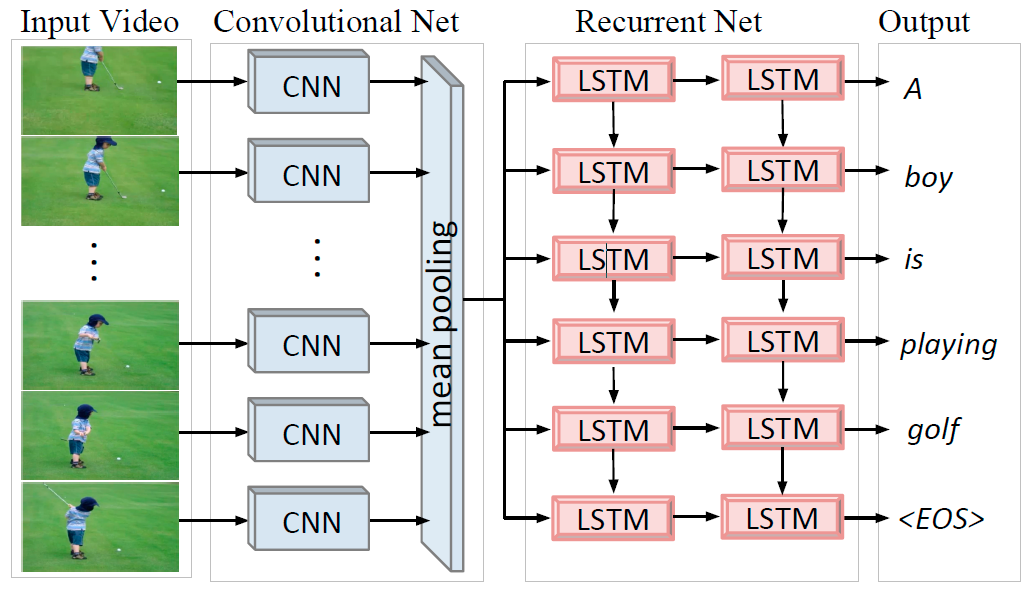
\includegraphics[width=11cm]{resources/mp.png}
\caption{Structure of video captioning system using mean pooling \cite{venugopalan2014translating}}
\label{fig:mp}
\end{figure}

Obviously, this approach fails to consider the temporal order of frames, and gives the same input to the decoder in every time step (as shown in the figure above). We can easily improve this model by replacing the arithmetic mean with weighted average \cite{yao2015describing}. Picture \ref{fig:sa} shows this structure.

\begin{figure}
\centering
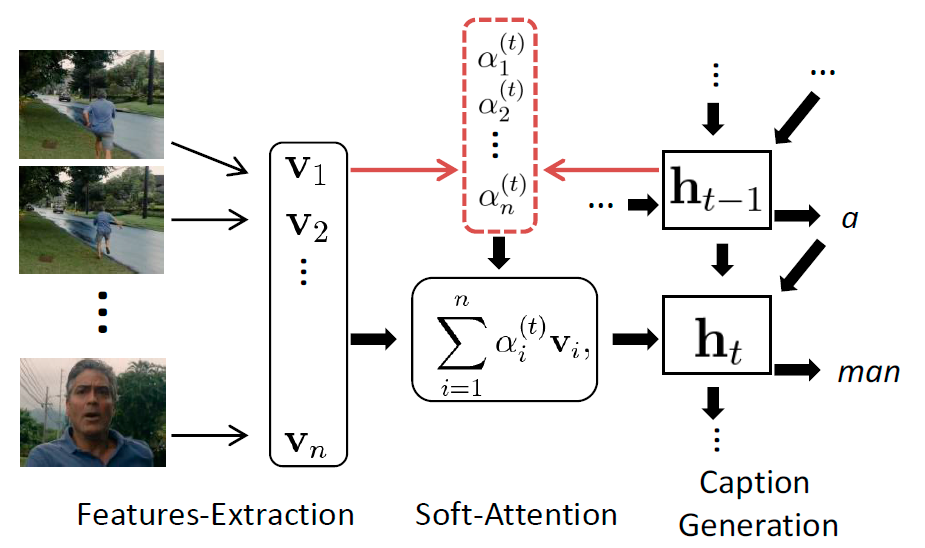
\includegraphics[width=11cm]{resources/sa.png}
\caption{Structure of video captioning system using temporal attention \cite{yao2015describing}}
\label{fig:sa}
\end{figure}

Ideally, we can let the model automatically choose the weights to attend on the most relevant set of frames when generating different words. These weights should be the function of current hidden state in RNN, conditioned on the CNN feature of frames.

\begin{equation}
e_{i}^{(t)} = f(v_i, h^{(t-1)})
\end{equation}

In this equation, $v_i$ represents a feature vector, and $h_{t-1}$ is the previous hidden state of which unit the weighted feature is going to input to. And assume $N$ is the number of frames and $T$ is the total number of time steps in RNN, we will have $i\in [1,N]$ and $t\in [1,T]$. (We can define $h^{(0)}$ as $\mathbf{0}$ vector so $t=1$ makes sense).

But this doesn't make sure $e_{i}^{(t)}$ will have a sum to 1 over all features (i.e. $\sum_{i=1}^Ne_i^{(t)}\neq 1$). So we apply softmax over them as follows.

\begin{equation}
\alpha_{i}^{(t)} = \frac{exp\{e_{i}^{(t)}\}}{\sum_{i=1}^Nexp\{e_{i}^{(t)}\}}
\end{equation}

This will give you $\sum_{i=1}^N\alpha_{i}^{(t)}=1$, so we can calculate a single feature for each time step as

\begin{equation}
\phi^{(t)}=\sum_{i=1}^N\alpha_{i}^{(t)}v_i
\end{equation}

So how we define $f(v_i,h^{(t)})$? That's much the similar of what we do in a node of neural. Just a linear function over $v_i$ and $h^{(t-1)}$ and add a non-linear activation function. Here we use $\tanh$ as the activation function.

\begin{equation}
e_{i}^{(t)} = w^T\tanh(W_ah^{(t-1)}+U_av_i+b_a)
\end{equation}
In which $w,W_a,U_a,b_a$ are all learnable parameters. Here we assume $r$ to be the size of an RNN hidden state, $m$ to be the encoding size of CNN, $a$ to be the attention matrix size (you can play with this parameter), we can list the size of those variables as follows

\begin{align}
v_i&\in \mathbb{R}^{m} \\
h^{(t)}&\in \mathbb{R}^{r}\\
W_a&\in \mathbb{R}^{a\times r}\\
U_a&\in \mathbb{R}^{a\times m}\\
b_a, w &\in \mathbb{R}^{a}
\end{align}
So this gives $e_i^{(t)}$ as a scalar value.

Another detail is that we share those learnable parameters both for different $i$ (features) and different $t$ (time steps), just like what RNN does. It can be implemented into the RNN unit so that the unit like LSTM can take a sequence as input. And as the equations are all differential, we can learn those parameters using back propagation with any optimization method.

This mechanism can definitely be used in other problems as long as you can transform the problem to a sequence representation. Theoretically, it will perform better than input a single item of a sequence because that can be described as a one-hot weight (i.e. weight over the sequence with a vector that only a single position takes 1 and others are all 0). However, if the attention matrix size $a$ is too small, intuitively, it won't cover all the possible weights to minimize the cost function, so the choice of $a$ is important.

\section{Experiment}
In this project, we explore several architectures of video captioning model. The implementation is based on NeuralTalk2\footnote{\url{https://github.com/karpathy/neuraltalk2}}. We mainly use MSR-VTT dataset \cite{xu2016msr}, but we are still planning to try our model on other datasets such as TGIF \cite{li2016tgif}.
\subsection{Dataset}
\paragraph{Microsoft Research - Video to Text (MSR-VTT)}
MSR-VTT provides 10K web video clips with 41.2 hours and 200K clip-sentence pairs in total, covering the most comprehensive categories and diverse visual content, and representing the largest dataset in terms of sentence and vocabulary. Each clip is annotated with about 20 natural sentences by 1,327 AMT workers. You can find a brief description of this dataset here\footnote{\url{https://github.com/chaonan99/chaonan99\_note/blob/master/paper/201609.md\#microsoft-research-video-to-text-msr-vtt}}. This is one of my works in the summer.

\paragraph{Tumblr GIF (TGIF)}
The Tumblr GIF (TGIF) dataset contains 100K animated GIFs and 120K sentences describing visual content of the animated GIFs. The animated GIFs have been collected from Tumblr, from randomly selected posts published between May and June of 2015. We provide the URLs of animated GIFs in this release. The sentences are collected via crowdsourcing, with a carefully designed annotation interface that ensures high quality dataset. We provide one sentence per animated GIF for the training and validation splits, and three sentences per GIF for the test split. The dataset shall be used to evaluate animated GIF/video description techniques. You can find a brief description of this dataset here\footnote{\url{https://github.com/chaonan99/chaonan99\_note/blob/master/paper/201609.md\#tumblr-gif-tgif}}.

\subsection{Models}
For all models, we use pre-trained VGG-16 \cite{simonyan2014very} network to generate frame level feature vector.
\paragraph{CNN encoder with meanpool}
The architecture is shown in Figure \ref{fig:mp}. We tried different hidden state size $r=256,512,1024$ and found $r=512$ performs best on MSR-VTT dataset. As the GPU of my computer has small memory, we set batch size as 1 and we only extract 15 frames for each video. We set learning rate to be $4e-4$ and tried two schedules. One is fixed learning rate, another is dividing the learning rate by 2 every 5000 iteration. We use adam optimizer \cite{Kingma2014Adam}. We found it little differences between two schedules. The model converge after 8\~9 epochs.

\paragraph{CNN encoder with attention}
The architecture is shown in Figure \ref{fig:sa}. We set hidden state size $r=512$ and we test different attention matrix size $a=256,512,1024$, and other settings the same as mean pooling model for comparison.

\paragraph{RNN encoder}
In s2vt \cite{venugopalan2015sequence} model, they use RNNs both in encoder and decoder, as shown in Figure \ref{fig:s2vt}. Yet they share parameters between encoder and decoder.

\begin{figure}
\centering
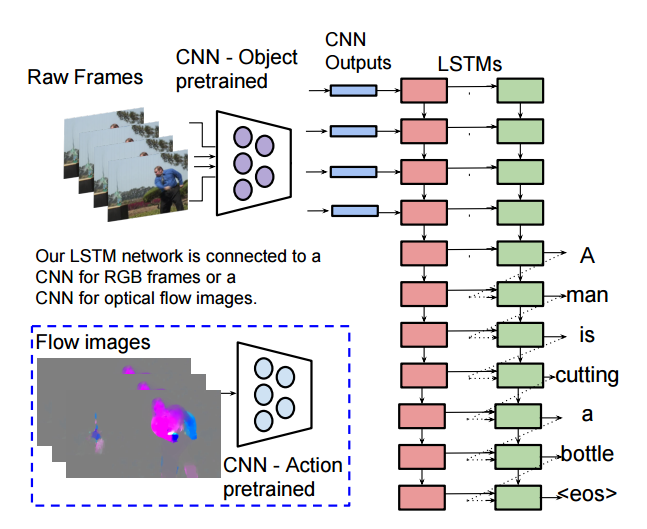
\includegraphics[width=11cm]{resources/s2vt.png}
\caption{S2vt model for video captioning \cite{venugopalan2015sequence}}
\label{fig:s2vt}
\end{figure}

Here we implement an RNN encoder model, but we separate encoder and decoder, i.e. do not share parameters between encoder and decoder RNN. We use two-layer LSTM as encoder and input frame features in each time step, and one-layer LSTM as decoder to generate caption. The model is shown in Figure \ref{fig:rnnenc}.

\begin{figure}[htbp]
\begin{minipage}[t]{0.5\linewidth}
\centering
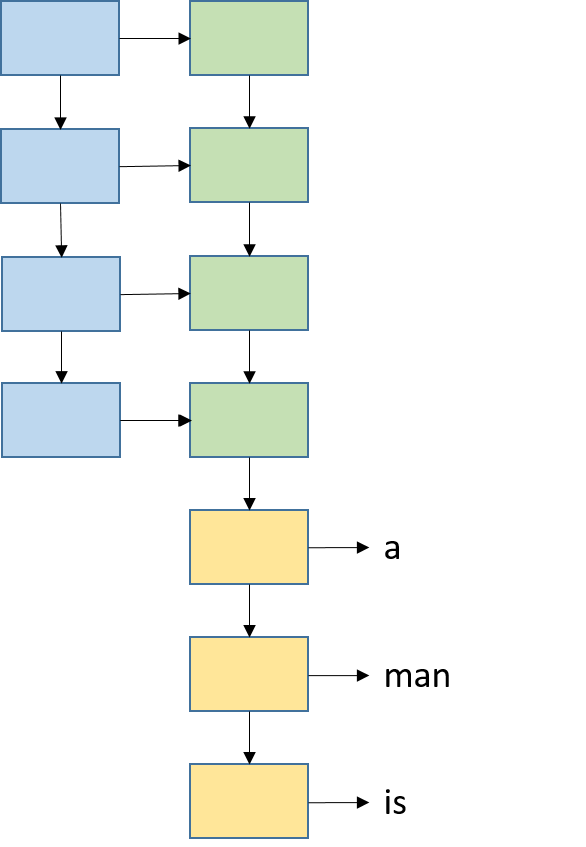
\includegraphics[width=1.4in]{resources/rnnenc.png}
\caption{RNN encoder}
\label{fig:rnnenc}
\end{minipage}
\begin{minipage}[t]{0.5\linewidth}
\centering
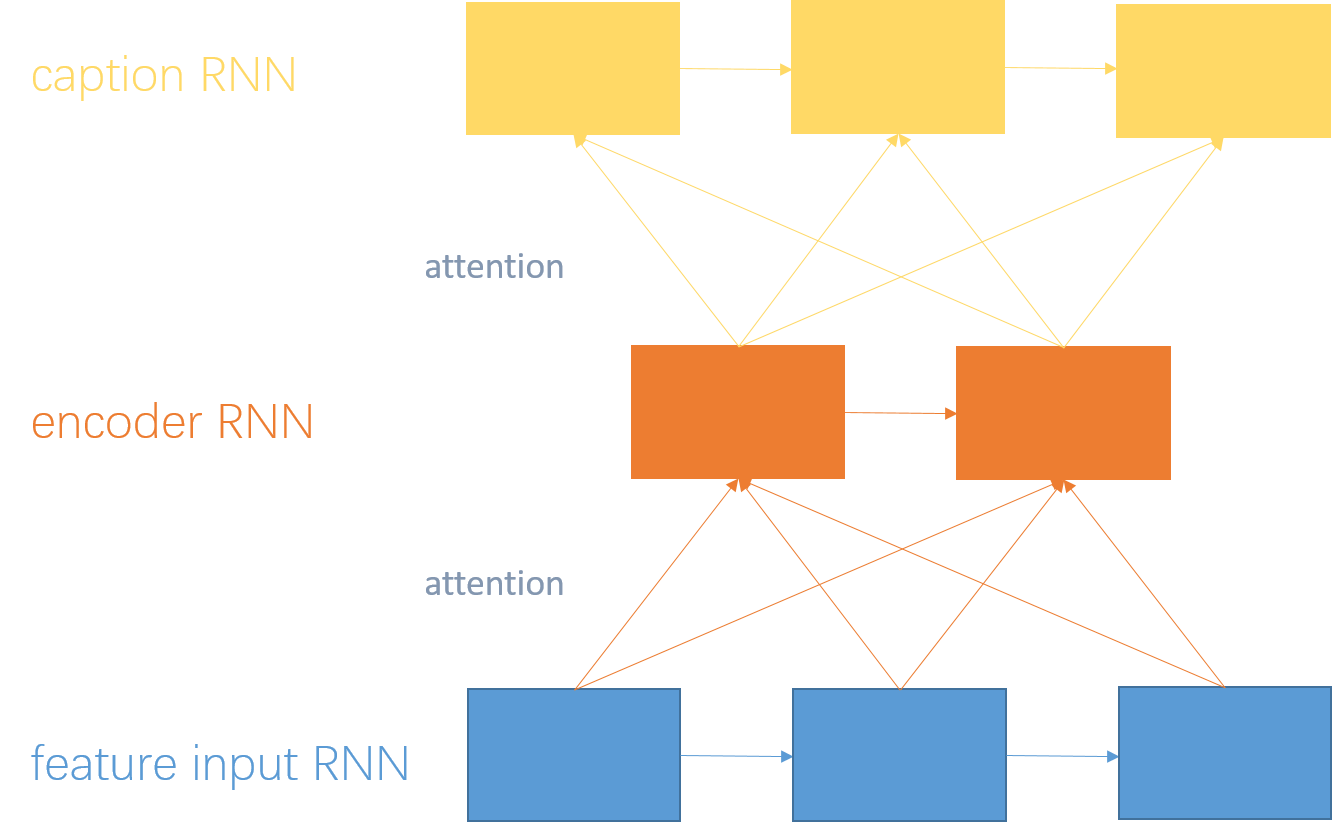
\includegraphics[width=3in]{resources/stack.png}
\caption{Stacked RNNs}
\label{fig:stack}
\end{minipage}
\end{figure}

\paragraph{Stacked LSTM}
As proposed in \cite{pan2015hierarchical}, we can use multiple layers LSTM to extract long-term temporal structure of a video. To verify its feasibility, we implement a model shown in Figure \ref{fig:stack}

\paragraph{Encoder with temporal segmentation}
We also propose a temporal segmentation layer shown in \autoref{fig:ts1} and \autoref{fig:ts2}. As pointed out in introduction section, videos in the wild always have several sceneries. To better handle long untrimmed video and extract their temporal structure, we attempt to divide frames into some groups and get a fixed representation for each group. The basic idea of temporal segmentation pipeline is as follows:

\begin{enumerate}
\item Concatenate CNN features of all frames.
\item Use different size of convolution kernels and get $L\times n$ vector, where $n$ is the number of kernels and $L$ is the number of feature vectors/frames. We assert this to be the score of segmentation proposal.
\item Select 10 top proposals to be the segmentation result.
\item We may use mean pooling or attention here to get a single feature vector for each split, and further feed all features into another RNN and do task on action recognition or video caption.
\end{enumerate}

The model use other segmentation model to provide ground truth. Thus it transfer the knowledge of segmentation model and are used on other task.

We have test this model on action recognition task and find it can improve the performance on UCF101 \cite{Soomro2012UCF101}. (This work is done by another group mate.) Currently we are conducting experiment on video captioning task.

\begin{figure}
\centering
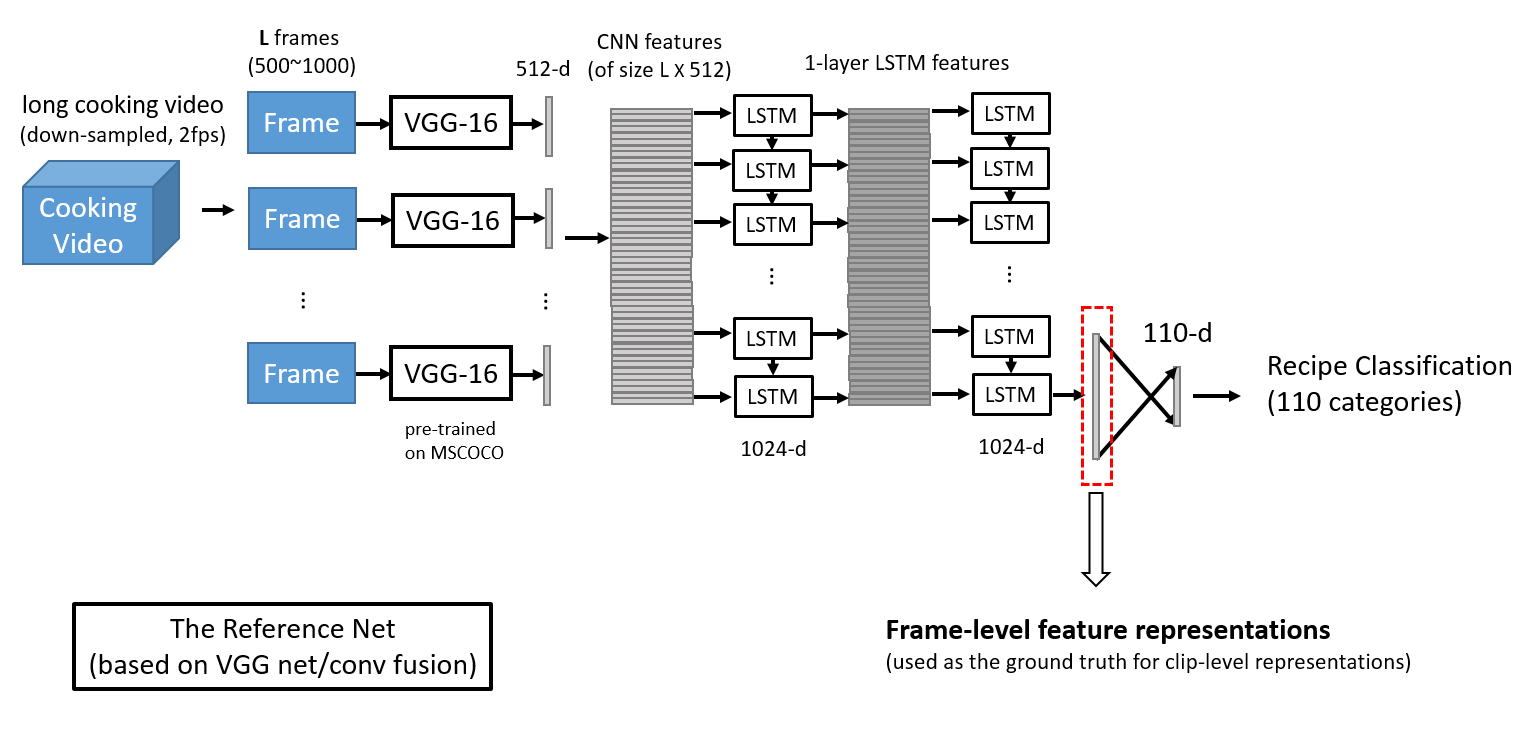
\includegraphics[width=15cm]{resources/ts1.png}
\caption{General encoder for video representation}
\label{fig:ts1}
\end{figure}

\begin{figure}
\centering
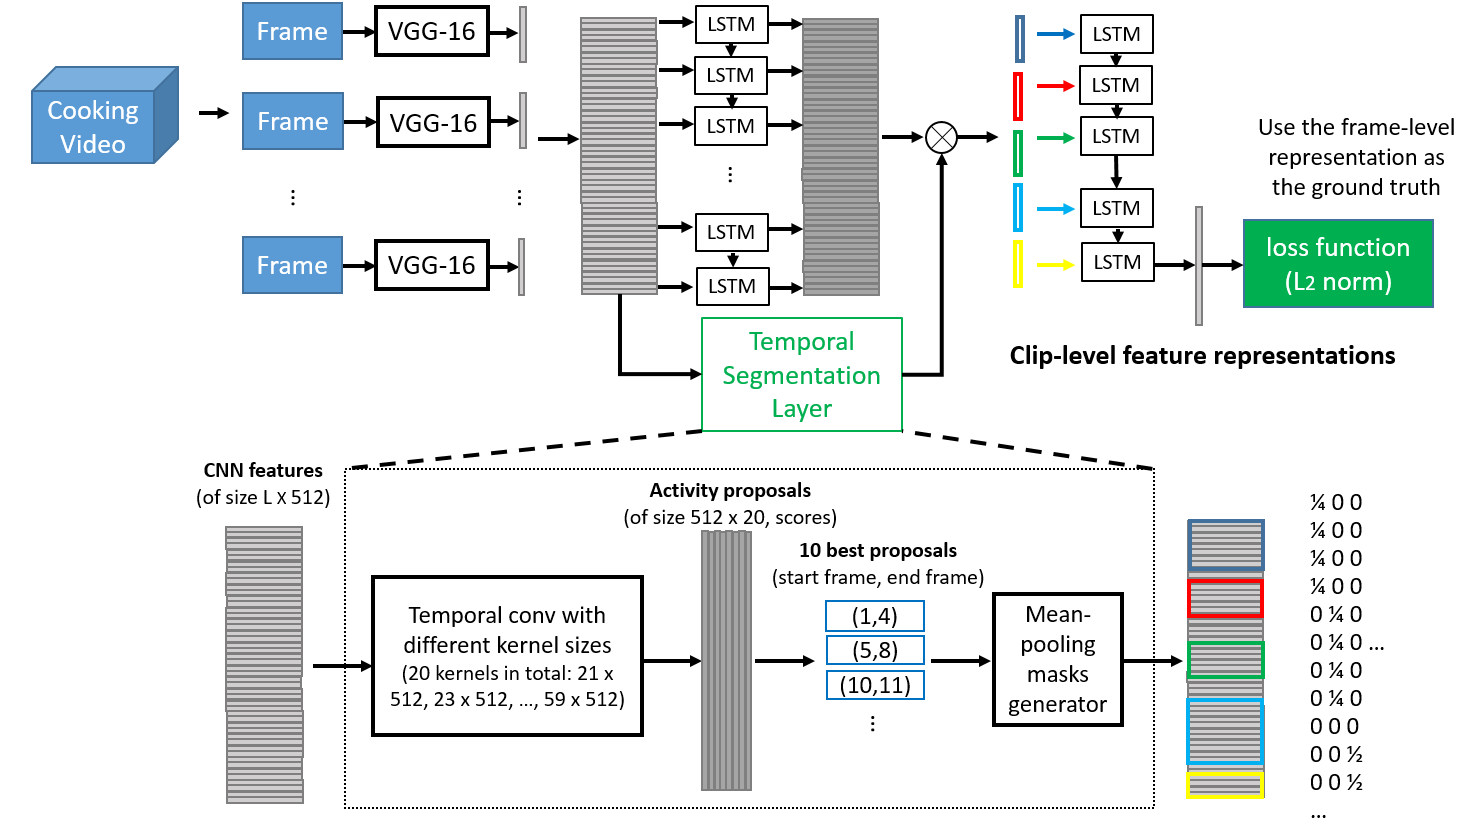
\includegraphics[width=15cm]{resources/ts2.png}
\caption{Encoder with temporal segmentation}
\label{fig:ts2}
\end{figure}

\subsection{Result and analysis}
\paragraph{Quantitative analysis}
\autoref{tab:res} shows the result of mean pooling model, attention based model and stacked RNN
\begin{table}[htbp]
  \centering
  \caption{Results of video caption models on MSR-VTT dataset}
    \begin{tabular}{lcccc}
    \toprule
          & \textbf{B@4\cite{Papineni2015BLEU}} & \textbf{R-L\cite{Lin2004Automatic}} & \textbf{METEOR\cite{Lavie2007METEOR}} & \textbf{CIDEr\cite{Vedantam2015CIDEr}} \\
    \midrule
    1-layer & 29.8  & 54.8  & 23.4  & 24.5 \\
    \textbf{2-layer, meanpool} & \textbf{34.6} & \textbf{56.8} & \textbf{25.5} & \textbf{32.1} \\
    2-layer, attention, 1024 & 32.4  & 56.2  & 24.3  & 26.6 \\
    \textbf{2-layer, attention, 512} & \textbf{34.7} & \textbf{57.1} & \textbf{25.4} & \textbf{30} \\
    2-layer, attention, 256 & 32.8  & 56    & 24.7  & 29.6 \\
    3-layer stacked RNN & 31.2  & 54.8  & 23.4  & 22.9 \\
    \bottomrule
    \end{tabular}
  \label{tab:res}
\end{table}

Note that attention based model only achieve equal performance with mean pooling model. We argue that this is because MSR-VTT only have one scenery in each video clip. In this case, attention model may not learn comprehensive long-term temporal structure. And as we only use 15 frames and set batch size to 1, the stacked RNN will easily overfitting thus yield bad performance.

\paragraph{Qualitative analysis}
We visualize the attention model to see what the model learned. As shown in \autoref{fig:att1} and \autoref{fig:att2}, different frames are attached with different range of weights.This suggest that the attention model has learned to differentiate between those frames.

\begin{figure}
\centering
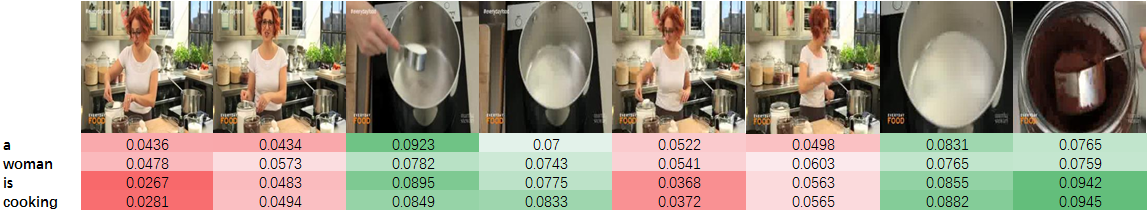
\includegraphics[width=14cm]{resources/att1.png}
\caption{Attention visualize for different frames. In this video, similar frames are given similar weights, thus the model learn to differentiate between those frames.}
\label{fig:att1}
\end{figure}

\begin{figure}
\centering
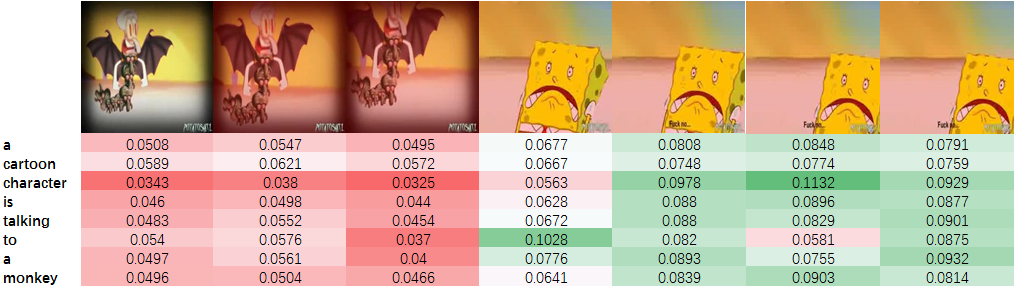
\includegraphics[width=14cm]{resources/att2.png}
\caption{Attention visualize for different frames, another example}
\label{fig:att2}
\end{figure}

As shown in \autoref{fig:att3}, the attention model may also change the weight according to the word it is generating.

\begin{figure}
\centering
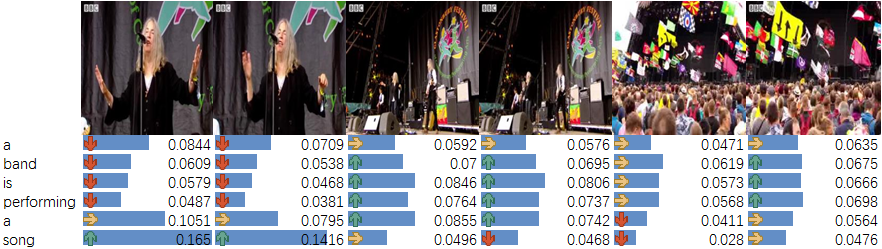
\includegraphics[width=14cm]{resources/att3.png}
\caption{Attention visualize showing changes for generating different words. When generating \lq{}\lq{}a band is performing\rq{}\rq{}, the model attend more on the latter four frames, which demonstrate the whole scenery of performing. When generating \lq{}\lq{}a song\rq{}\rq{}, the model attend more on the former two frames, which demonstrate a person singing something.}
\label{fig:att3}
\end{figure}

\section{Related works}
\subsection{Image captioning with RNNs}
Automatically generating a natural language description of an image, a problem known as image captioning, has recently received a lot of attention in Computer Vision. The problem is interesting not only because it has important practical applications, such as helping visually impaired people see, but also because it is regarded as a grand challenge for image understanding which is a core problem in Computer Vision. The first attempt of visual to text translation using RNNs was seen in the work of image captioning \cite{Mao2014Deep,Vinyals2015Show} which can be treated as a special case of video captioning when each video has a single frame and no temporal structure. This is inspired by the success of using encoder-decoder framework in neural machine translation (NMT) task \cite{cho2014learning}. From then on, there are many attempt on image caption generation. \cite{xu2015show} use attention mechanism on image captioning task, also inspired by attention mechanism on NMT \cite{bahdanau2014neural}. \cite{Jia2015Guiding} use semantic information as guidance to train the decoder. They calculate the correlation between image and its description using canonical correlation analysis. \cite{You2016Image} explore the structure of language and combine image-to-text embedding and text-to-image embedding together. They introduce a feedback in general encoder-decoder framework.

\subsection{Video captioning with RNNs}
Early work of video captioning \cite{venugopalan2014translating} based on RNNs extends the image captioning methods by simply average pooling the video frames. However, this strategy works only for short video clips where there is only one major event, usually appearing in one video shot from the beginning to the end. To avoid this issue, more sophisticated ways of encoding video features were proposed in later work, using either a recurrent encoder \cite{donahue2015long,venugopalan2015sequence,xu2015multi} or an attention model \cite{yao2015describing}. Also some recent work attempt to extract long-term temporal structure of a video. \cite{pan2015hierarchical} use a hierarchical RNN model to summarize video feature in different time scale. \cite{yu2015video} proposes a model to generate paragraph description for long video.

\section{Web interface}
During this summer, I'm also working on the video to text website\footnote{\url{http://www.videototext.net/}}. The website work flow is shown in \autoref{fig:web}. The website is developed using Flask and runs on Apache http server. It also use Celery to provide task pipeline and use MySQL database to store suggested caption. The interface is shown in \autoref{fig:int}.

\begin{figure}
\centering
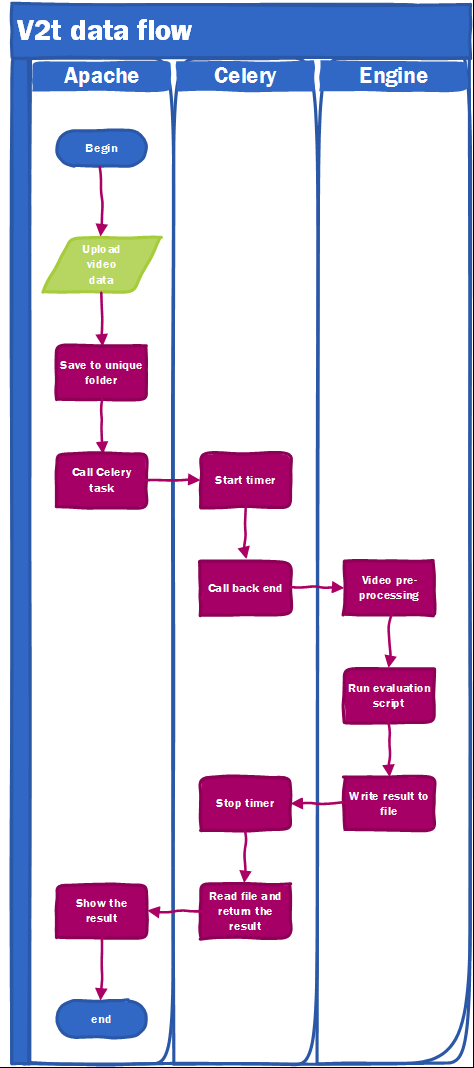
\includegraphics[width=8cm]{resources/web.png}
\caption{Website work flow}
\label{fig:web}
\end{figure}

\begin{figure}
\centering
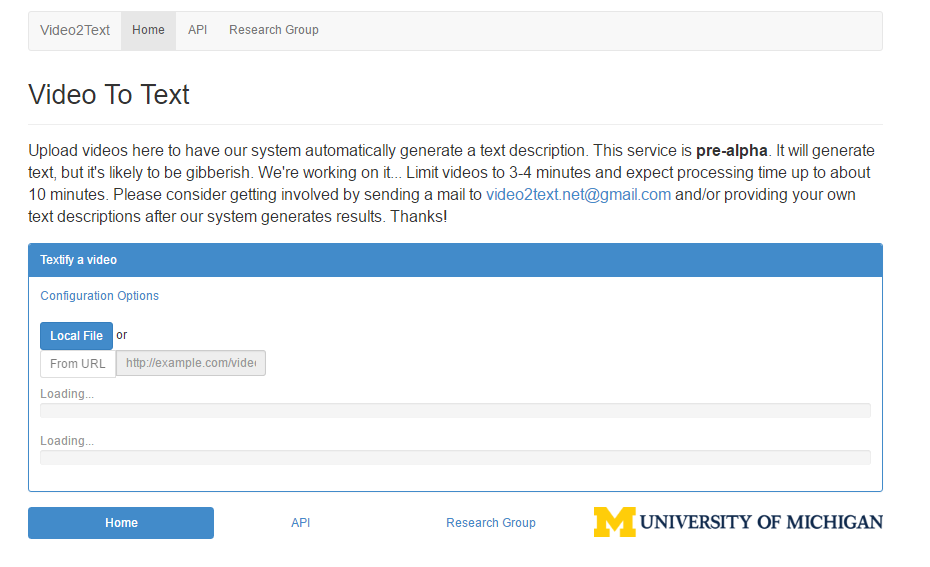
\includegraphics[width=8cm]{resources/int.png}
\caption{Website work flow}
\label{fig:int}
\end{figure}

\section{Future works}
We are still working on this project, especially using temporal segmentation in video caption task and compare with attention based model.

\section{Acknowledgment}
This work is carried out in computer vision lab, University of Michigan, Ann Arbor, US under the guidance of Prof. Jason Corso, with the help of his PhD student, Luowei Zhou.

\bibliography{reference}

\end{document}
